\chapter{Testing}

To check the accuracy and performance of the add-on, we created different variants of Transcriptase malware.

\section{Generating Transcriptase variants}

Transcriptase was written in JScript, so in windows system it can be executed by simply double clicking it. Generation of each version takes around 15 minutes. 

As explained in Section \ref{transcriptasesection}, Transcriptase carries its source code as meta instructions and on each execution it creates different variant of its JS source, then prepends that JS code to all the JavaScript files in its directory. So, I followed the below steps to create 100 versions:
\begin{enumerate}
\item Created an empty JavaScript file in Transcriptase directory
\item Executed Transcriptase, which infects the new empty JavaScript file and converts it to another variant of Transcriptase
\item Move the older version Transcriptase (or creator Transcriptase) to different folder.
\item Then created an empty JavaScript file in the current folder where the new Transcriptase variant exists.
\item Executed the new variant to infect the empty JavaScript file. Go to Step 3 if required number of variants aren`t generated. 
\end{enumerate}
Code in Figure \ref{fig:batchscriptcode} automates the above mentioned steps.

\begin{figure}[h]
  \centering
\begin{lstlisting}[frame=single,language=JavaScript,mathescape=false,morekeywords={REN, MOVE, IN, COPY, PAUSE, FOR, DO}]
FOR %%A IN (1 2 3 4 5 6 7 8 9 10 11 12 13 14 15 16 17 18 19 20 21 22 23 24 25 26 27 28 29 30 31 32 33 34 35 36 37 38 39 40 41 42 43 44 45 46 47 48 49 50 51 52 53 54 55 56 57 58 59 60 61 62 63 64 65 66 67 68 69 70 71 72 73 74 75 76 77 78 79 80 81 82 83 84 85 86 87 88 89 90 91 92 93 94 95 96 97 98 99 100) DO (
transcriptase.js
REN transcriptase.js "var%%~nA.*"
MOVE "var%%~nA.*" "C:\Users\Sravan\Downloads\Transcriptase\versions"
REN empty.js transcriptase.js
COPY "C:\Users\Sravan\Downloads\Transcriptase\template\empty.js" .
)
PAUSE
\end{lstlisting}
\caption[Batch script]{Batch script that automates the Transcriptase variants generations}
    \label{fig:batchscriptcode}
\end{figure}

\begin{figure}[h]
  \centering
      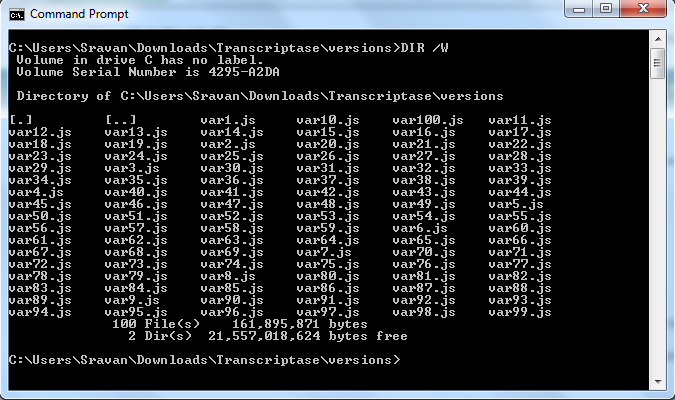
\includegraphics[width=13.5cm, height=8cm]{Capture.PNG}
    \caption[Transcriptase`s 100 versions]{Transcriptase`s 100 versions.}
    \label{fig:100versions}
\end{figure}

\LaTeX\ can be viewed
as a compiled programming language, in contrast to that 
nightmare known as Microsoft Word,
which can be viewed as an interpreted language. So, to typeset a
document in \LaTeX, you create a text file that has the {\tt .tex} extension.
This file includes some special
commands, known as macros. Then
you compile your {\tt .tex} file by running  \LaTeX,
which produces your typeset document, as a pdf. 

In this paper, a few basics are discussed. There are plenty of good online resource
if you need help with more advanced topics.


\section{Accuracy} 

To typeset text, you type whatever you want. Multiple spaces are
ignored                           when typesetting, and
the end of a line is treated as another space.
Consequently, when you are typing, you can break lines anywhere, like here
or here,
since the lines are formatted automatically when you typeset the document.
You start a new paragraph by leaving a blank line.

See how easy it is to start a new paragraph? A blank line does the trick.


\section{Performance}

Typesetting text is generally pretty easy. However, there are some special
characters that will not be typeset as you might expect. In the remainder of this
section we consider some of the most common of these
special characters. 

The backslash ``\verb+\+'' is used 
as the ``escape'' character, meaning that
whatever follows a backslash is interpreted as a macro.
For example, when \verb+\LaTeX+ is typeset, it looks like \LaTeX, which 
is a lot different from LaTeX.

To get double quotes, use two single quotes. That is, the left double quote is ``, while the right double
quote is ''. When you do it correctly, quoted text looks ``like this.''
If you use the double quote key, you will always get right-quotes, which looks "like this," and is
almost certainly not what you want.

A tilde ``\verb+~+'' is used as a ``tie,'' that is, a space is inserted, but no line break can occur.
For example, you might type Dr.~Stamp just to be sure that the line of text
does not break between Dr. and Stamp, as it otherwise might.

The percent sign is used for comments---everything following a percent sign 
on a given line is ignored when you \LaTeX\ your file. % Like this stuff here
If you want a percent sign to appear in your document, use \verb+\%+, 
which will give you this \%.

The dollar sign also has special meaning, since it is used to start and end
math formulas. To typeset a dollar sign, use \verb+\$+, like this~\$.

To force \LaTeX\ to insert a space, use a backslash followed by
a space, that is, \verb+\ +. You can put in multiple extra spaces\ \ \ \ \ \ \ if you want.

